\documentclass[12pt,aspectratio=169]{beamer}

\usetheme[
    sectionpage=progressbar,
    subsectionpage=progressbar,
    progressbar=frametitle
]{metropolis}

\usefonttheme{professionalfonts}

\definecolor{blue-grey-900}{HTML}{263238}
\definecolor{deep-orange-500}{HTML}{FF5722}
\setbeamercolor{normal text}{fg=blue-grey-900, bg=white}
\setbeamercolor{alerted text}{fg=deep-orange-500}

\usepackage{booktabs}
\usepackage{graphicx}
\usepackage{hyphenat}

\usepackage{polyglossia}
\setdefaultlanguage[variant=british]{english}
\usepackage[english=british]{csquotes}

\usepackage{fontspec}
\setmainfont{Lucida Sans OT}
\setsansfont[Scale=MatchLowercase]{Lucida Sans OT}
\setmonofont[Scale=MatchLowercase]{Lucida Console DK}
\defaultfontfeatures{Ligatures=TeX}

\usepackage[mathbf=sym]{unicode-math}
\setmathfont{TeX Gyre Pagella Math}

\newcommand{\set}[1]{\ensuremath{\mathcal{#1}}}

\renewcommand{\vec}[1]{\ensuremath{\mathbf{#1}}}
\newcommand{\mat}[1]{\ensuremath{\vec{#1}}}
\newcommand{\tr}{\ensuremath{\intercal}}

\newcommand{\R}{\ensuremath{\mathbb{R}}}
\newcommand{\N}{\ensuremath{\mathcal{N}}}

\title{Follow the gradient}
\subtitle{An introduction to mathematical optimisation}
\author{Gianluca Campanella}
\date{27\textsuperscript{th} April 2018}

\begin{document}

\maketitle

\begin{frame}{Contents}
    \tableofcontents
\end{frame}

\section{Optimisation}

\begin{frame}{What is optimisation?}
    \begin{description}
        \item[Have] An objective function, e.g.\ $f\,:\,\R^{p} \to \R$
        \item[Want] The optimal $\vec{x}^{\star}$ that minimises (or maximises)
                    $f$
    \end{description}
    \vfill
    \begin{block}{Why?}
        \begin{itemize}
            \item $f$ represents some goal, e.g.\ error to be minimised
            \item Want the `best' element from some set of available
                  alternatives
        \end{itemize}
    \end{block}
\end{frame}

\begin{frame}[t]{Optimisation in ML}
    \begin{itemize}
        \item Many ML methods are defined in terms of a \alert{loss function}
        \item[$\to$] Really optimisation problems!
    \end{itemize}
    \vfill
    \only<2>{%
        \begin{block}{Linear regression}
            \begin{align*}
                \operatorname{MSE}\!\left( \left. \hat{\vec{\beta}} \,\right| \mat{X}, \vec{y} \right) &= \frac{1}{n} \sum_{i} \left( \hat{y}_{i} - y_{i} \right)^{2} \\
                \hat{y}_{i} &= \vec{x}_{i}\,\hat{\vec{\beta}}
            \end{align*}
        \end{block}}
    \only<3>{%
        \begin{block}{Logistic regression}
            \begin{align*}
                \operatorname{LogLoss}\!\left( \left. \hat{\vec{\beta}} \,\right| \mat{X}, \vec{y} \right) &= - \sum_{i} \left[ y_{i} \log \hat{p}_{i} + (1 - y_{i}) \log (1 - \hat{p}_{i}) \right] \\
                \hat{p}_{i} &= \operatorname{logit}^{-1}(\vec{x}_{i}\,\hat{\vec{\beta}})
            \end{align*}
        \end{block}}
\end{frame}

\begin{frame}{Types of optimisation problems}
    \begin{align*}
        f_{1}(\vec{x}) \in \R \text{,} \quad & \vec{x} \in \R^{100} \\[\medskipamount]
        f_{2}(\vec{x}) \in \R \text{,} \quad & \vec{x} \in \R^{100} \text{,} \quad \vec{1}^{\tr} \vec{x} = 1 \\[\medskipamount]
        f_{3}(\vec{x}) \in \R \text{,} \quad & \vec{x} \in \{0, 1\}^{100}
    \end{align*}
    \vfill
    \begin{block}{Question}
        Which is `harder' to optimise, and why?
    \end{block}
\end{frame}

\begin{frame}{Standard form}
    \begin{align*}
        \min_{\vec{x}} \quad& f(\vec{x}) \\
        \mathup{s.t.}  \quad& g_{j}(\vec{x}) \leq 0,       \quad j = 1, \ldots, m \\
                            & h_{k}(\vec{x}) = 0,          \quad k = 1, \ldots, n \\
                            & l_{i} \leq x_{i} \leq u_{i}, \quad i = 1, \ldots, p
    \end{align*}
    \vfill
    \begin{itemize}
        \item $\vec{x}$ can be continuous or discrete
        \item $f$ can be linear or nonlinear, explicit or implicit
    \end{itemize}
\end{frame}

\begin{frame}{Combinatorial optimisation}
    \begin{itemize}
        \item Combinatorial problems like optimising $f_{3}$ are intrinsically
              hard
        \item[$\to$] Need to try all $2^{100} \approx 1.27 \times 10^{30}$
                     combinations
    \end{itemize}
    \vfill
    \begin{block}{Side note}
        \begin{itemize}
            \item Solving for $\vec{x} \in [0, 1]^{100}$ is easier
                  (assuming $h$ is continuous)
            \item[$\to$] Approximate solution (relaxation)
        \end{itemize}
    \end{block}
\end{frame}

\begin{frame}{Continuous optimisation}
    \only<1>{
        \begin{center}
            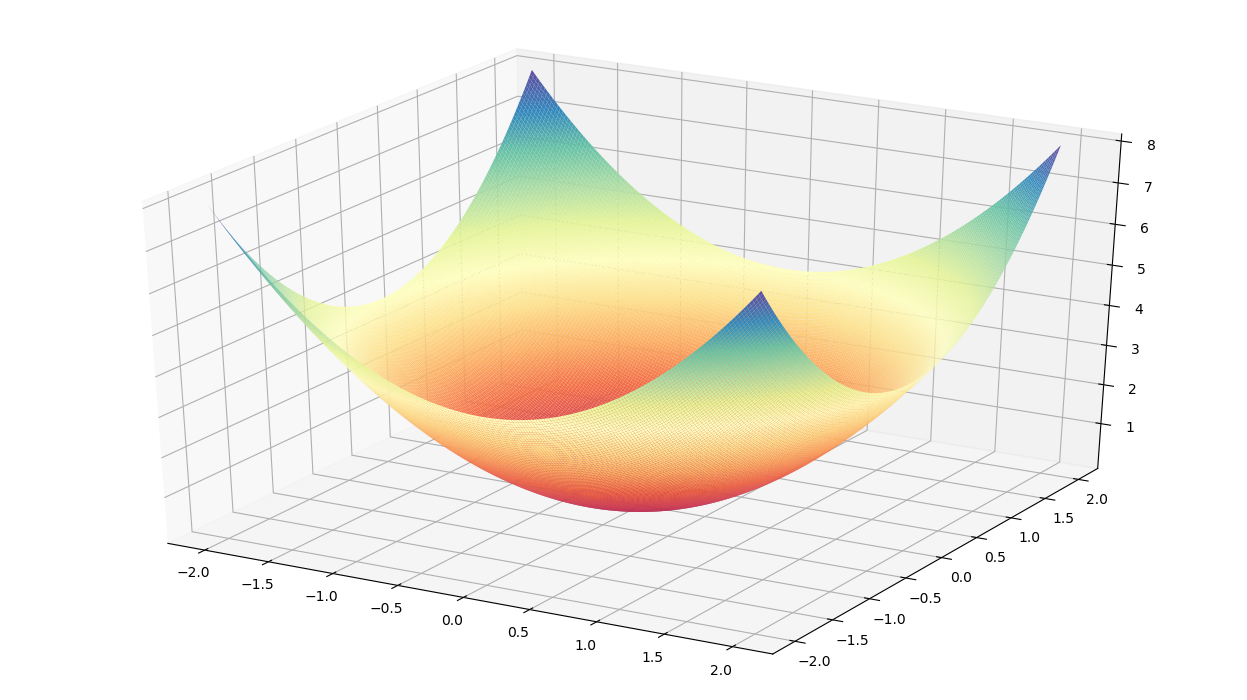
\includegraphics[height=0.85\textheight]{figures/sphere_fun}
        \end{center}}
    \only<2>{
        \begin{center}
            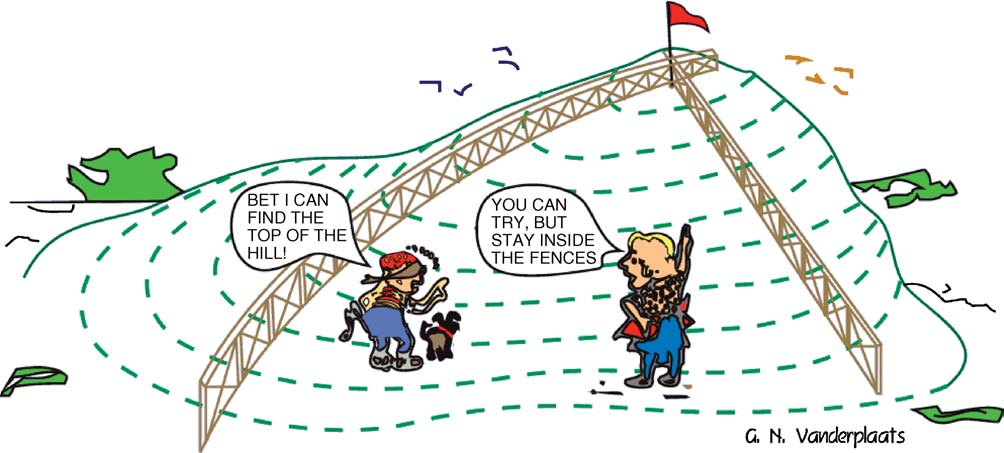
\includegraphics[height=0.8\textheight]{figures/hill_climbing} \\
            {\scriptsize%
             From G.\ Venter (originally from G.\ N.\ Vanderplaats)}
        \end{center}}
    \only<3>{
        \begin{center}
            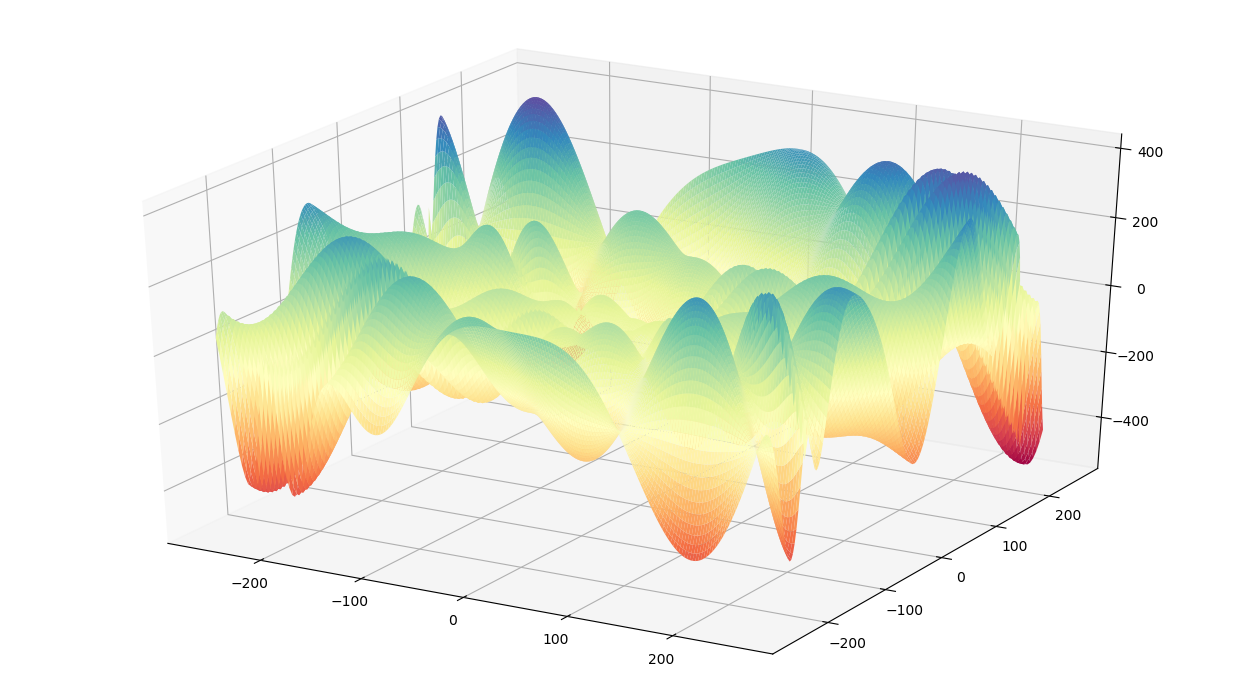
\includegraphics[height=0.85\textheight]{figures/eggholder_fun}
        \end{center}}
\end{frame}

\begin{frame}{Convex functions}
    \begin{columns}
        \begin{column}{0.5\textwidth}
            \centering
            Function is \alert{convex} \\[1em]
            $\downarrow$ \\[1em]
            Any local minimum is \\ also a global minimum
        \end{column}
        \begin{column}{0.5\textwidth}
            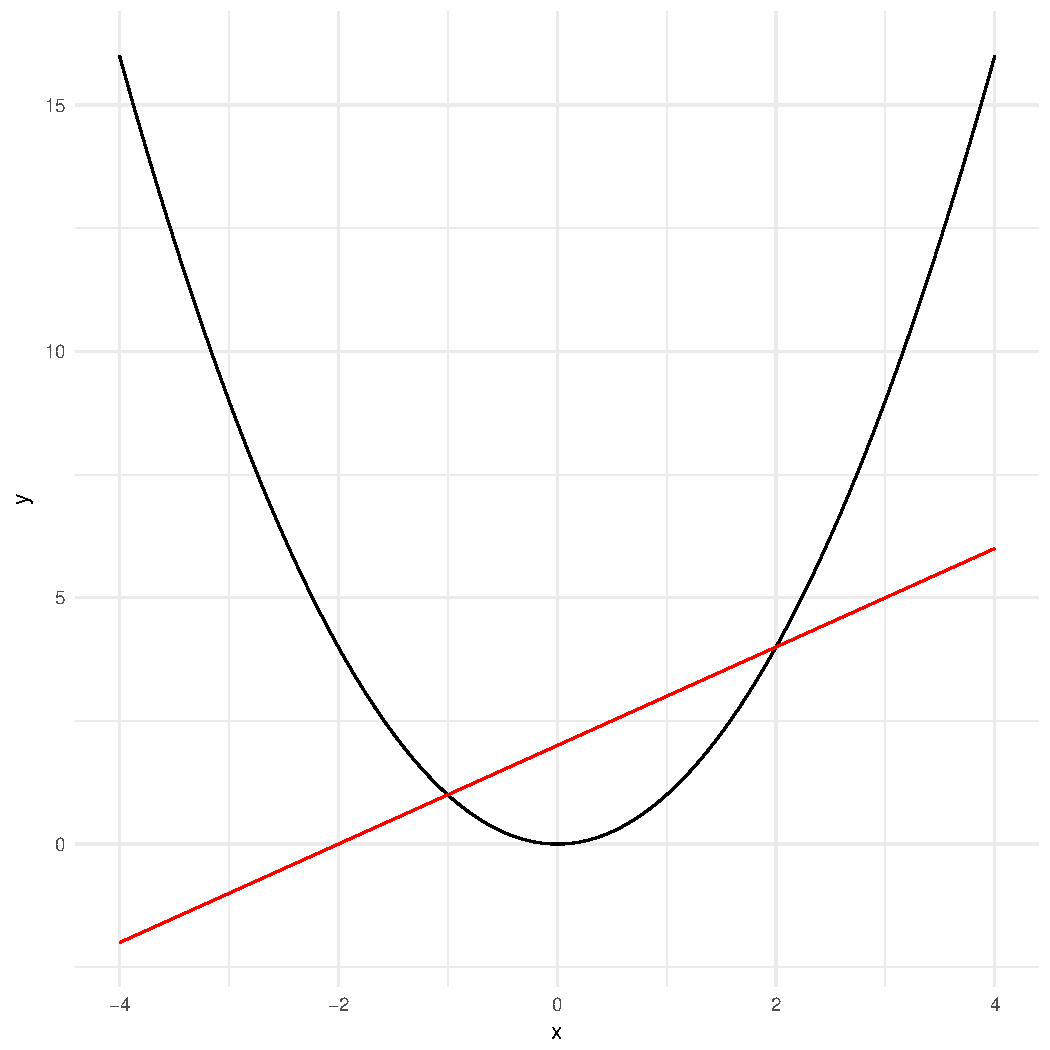
\includegraphics[height=0.85\textheight]{figures/convex_fun}
        \end{column}
    \end{columns}
\end{frame}

\section{Linear programming}

\begin{frame}{Linear programs}
    \begin{columns}
        \begin{column}{0.5\textwidth}
            \begin{align*}
                \max_{\vec{x}}    \quad& \vec{c}^{\tr} \vec{x} \\
                \mathnormal{s.t.} \quad& \mat{A} \vec{x} \leq \vec{b} \\
                                  \quad& \vec{x} \geq \vec{0}
            \end{align*}
        \end{column}
        \begin{column}{0.5\textwidth}
            \begin{block}{Properties}
                \begin{itemize}
                    \item Linear objective
                    \item Linear constraints
                \end{itemize}
            \end{block}
            \vfill
            \begin{block}{Types of solution}
                \begin{itemize}
                    \item Optimal
                    \item Infeasible
                    \item Unbounded
                \end{itemize}
            \end{block}
        \end{column}
    \end{columns}
\end{frame}

\begin{frame}{Graphical solution}
    \begin{columns}
        \begin{column}{0.5\textwidth}
            \begin{align*}
                \max_{\vec{x}}    \quad& 3 x_{1} + 4 x_{2} \\
                \mathnormal{s.t.} \quad& x_{1} + 2 x_{2} \leq 14 \\
                                       & 3 x_{1} - x_{2} \geq 0 \\
                                       & x_{1} - x_{2} \leq 2
            \end{align*}
        \end{column}
        \begin{column}{0.5\textwidth}
            \centering%
            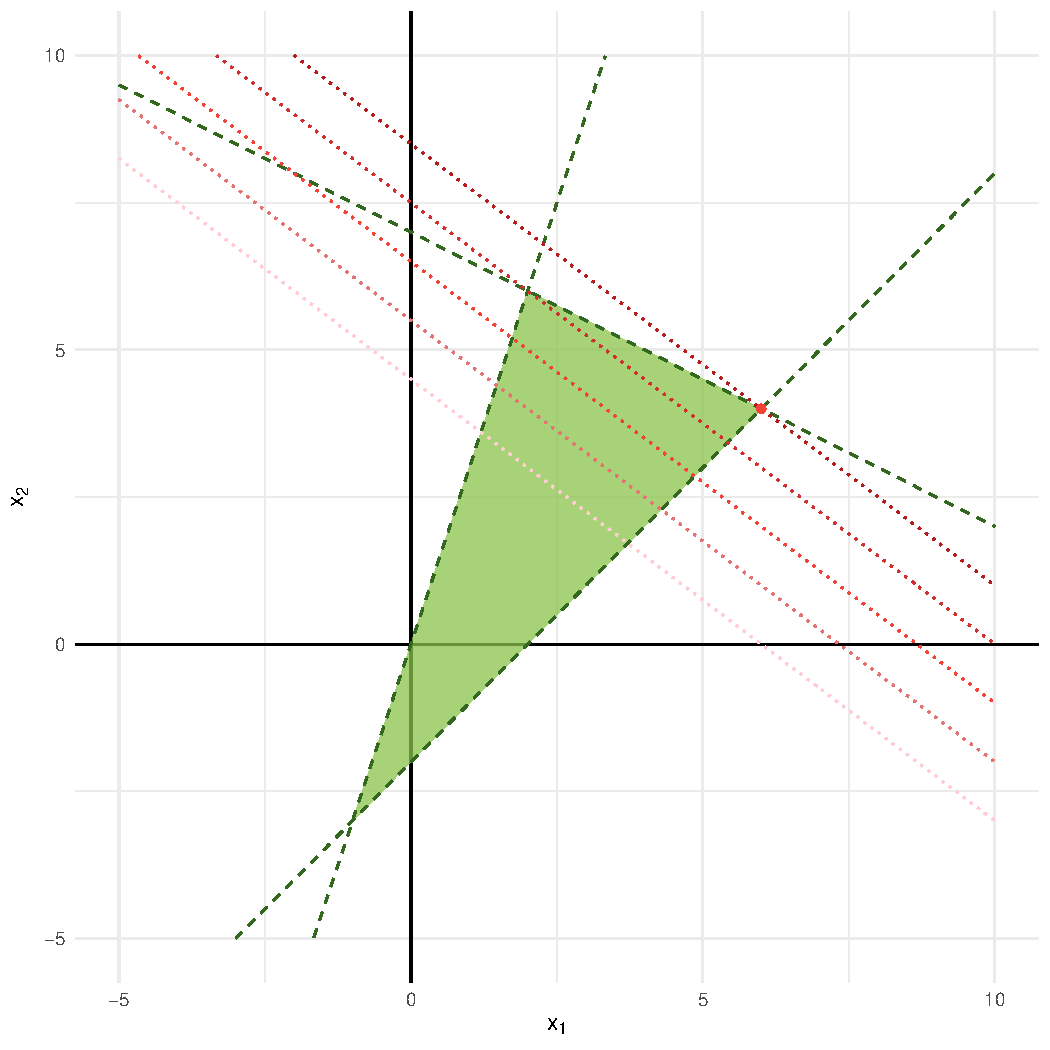
\includegraphics[width=\textwidth]{figures/lp}
        \end{column}
   \end{columns}
\end{frame}

\begin{frame}{LAD regression problem}
    We can rewrite the LAD (robust) regression problem
    \[
        \min_{\vec{\beta}} \ \left|\left|\,\mat{X}\vec{\beta} - \vec{y}\,\right|\right|_{1}
        = \sum_{i} \left| \varepsilon_{i} \right|
    \]
    as the linear program
    \begin{columns}
        \begin{column}{0.475\textwidth}
            \begin{align*}
                \min_{\vec{\beta},\,\vec{t}} \quad& \vec{1}_{n}^{\tr} \vec{t} \\
                \mathnormal{s.t.}            \quad& -\vec{t} \leq \mat{X} \vec{\beta} - \vec{y} \leq \vec{t} \\
                                                  & \vec{t} \in \R^{n}
            \end{align*}
        \end{column}
        \begin{column}{0.05\textwidth}
            \centering%
            or
        \end{column}
        \begin{column}{0.475\textwidth}
            \begin{align*}
                \min_{\vec{\beta},\,\vec{u},\,\vec{v}} \quad& \vec{1}_{n}^{\tr} \vec{u} + \vec{1}_{n}^{\tr} \vec{v} \\
                \mathnormal{s.t.}                      \quad& \mat{X} \vec{\beta} + \vec{u} - \vec{v} = \vec{y} \\
                                                            & \vec{u}, \vec{v} \geq \vec{0}
            \end{align*}
        \end{column}
    \end{columns}
\end{frame}

\begin{frame}{$\tau^{\text{th}}$ quantile regression problem}
    \begin{align*}
        \min_{\vec{\beta},\,\vec{u},\,\vec{v}} \quad& \alert{\tau}\,\vec{1}_{n}^{\tr} \vec{u} + \alert{(1 - \tau)} \vec{1}_{n}^{\tr} \vec{v}, \quad \tau \in [0, 1] \\
        \mathnormal{s.t.}                      \quad& \mat{X} \vec{\beta} + \vec{u} - \vec{v} = \vec{y} \\
                                                    & \vec{u}, \vec{v} \geq \vec{0}
    \end{align*}
    \vfill
    \begin{itemize}
        \item $\tau = 0.5$ recovers the LAD regression problem
        \item Very efficient (custom) algorithms exist
    \end{itemize}
\end{frame}

\section{Convex programming}

\begin{frame}{Convex quadratic programs}
    \begin{columns}
        \begin{column}{0.5\textwidth}
            \begin{align*}
                \min_{\vec{x}}    \quad& \frac{1}{2} \vec{x}^{\tr} \mat{Q} \vec{x} + \vec{c}^{\tr} \vec{x} \\
                \mathnormal{s.t.} \quad& \mat{A} \vec{x} \preceq \vec{b} \\
                                       & \vec{x} \succeq \vec{0}
            \end{align*}
        \end{column}
        \begin{column}{0.5\textwidth}
            \begin{block}{Properties}
                \begin{itemize}
                    \item Quadratic objective
                    \item Quadratic constraints
                \end{itemize}
            \end{block}
            \vfill
            \begin{block}{Question}
                Does quadratic imply convex?
            \end{block}
        \end{column}
    \end{columns}
\end{frame}

\begin{frame}{OLS regression problem}
    \only<1>{%
        We can rewrite the OLS regression problem
        \[
            \min_{\vec{\beta}} \ \left|\left|\,\mat{X}\vec{\beta} - \vec{y}\,\right|\right|_{2}^{2}
            = \sum_{i} \varepsilon_{i}^{2}
        \]
        as the convex quadratic objective
        \[
            f(\vec{\beta}) = \vec{\beta}^{\tr} \mat{X}^{\tr} \mat{X} \vec{\beta} - 2 \vec{y}^{\tr} \mat{X} \vec{\beta} + \vec{y}^{\tr} \vec{y}
        \]}
    \only<2>{%
        Setting the gradient to 0 and solving for $\vec{\beta}$\ldots
        \begin{align*}
            \nabla f = 2 \mat{X}^{\tr} \mat{X} \vec{\beta} - 2 \mat{X}^{\tr} \vec{y} &= 0 \\
            \mat{X}^{\tr} \mat{X} \vec{\beta} &= \mat{X}^{\tr} \vec{y} \\
            \hat{\vec{\beta}} &= \left( \mat{X}^{\tr} \mat{X} \right)^{-1} \mat{X}^{\tr} \vec{y}
        \end{align*}}
\end{frame}

\begin{frame}{Ridge regularisation}
    \[
        \min_{\vec{\beta}} \ \left|\left|\,\mat{X}\vec{\beta} - \vec{y}\,\right|\right|_{2}^{2}
        + \alert{\lambda \left|\left|\, \vec{\beta} \,\right|\right|_{2}^{2}},
        \quad
        \lambda \geq 0
    \]
    \vfill
    The objective becomes\ldots
    \[
        f(\vec{\beta}) = \vec{\beta}^{\tr} \left( \mat{X}^{\tr} \mat{X} + \alert{\lambda \mat{I}_{p}} \right) \vec{\beta} - 2 \vec{y}^{\tr} \mat{X} \vec{\beta} + \vec{y}^{\tr} \vec{y}
    \]
\end{frame}

\begin{frame}{Constraints on $\vec{\beta}$}
    \centering%
    \begin{tabular}{ll}
        \toprule
        \textbf{Condition} & \textbf{Useful for\ldots} \\
        \midrule
        $\vec{\beta} \geq \vec{0}$ & Intensities or rates \\
        $\vec{l} \leq \vec{\beta} \leq \vec{u}$ & Knowledge of permissible values \\
        $\vec{\beta} \geq \vec{0} \land \vec{1}^{\tr}_{p} \vec{\beta} = \vec{1}$ & Proportions and probability distributions \\
        \bottomrule
    \end{tabular}
\end{frame}

\section{Follow the gradient}

\begin{frame}{Why follow the gradient?}
    \begin{center}
        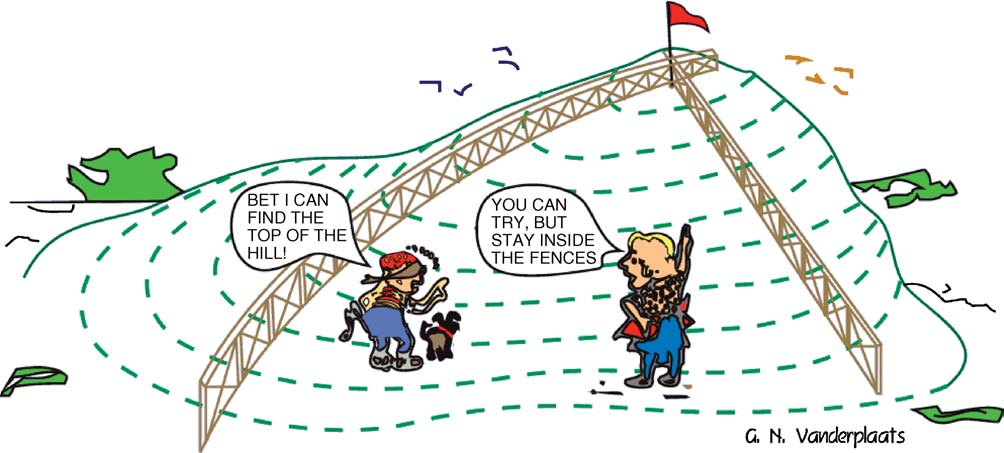
\includegraphics[height=0.8\textheight]{figures/hill_climbing} \\
        {\scriptsize%
         From G.\ Venter (originally from G.\ N.\ Vanderplaats)}
    \end{center}
\end{frame}

\begin{frame}{Karush-Kuhn-Tucker conditions}
    \begin{enumerate}
        \setlength{\itemsep}{\bigskipamount}
        \item $\vec{x}^{\star}$ is feasible
        \item The gradient of the Lagrangian vanishes at $\vec{x}^{\star}$
              \[
                  \nabla f(\vec{x}^{\star}) +
                  \sum_{j = 1}^{m} \lambda_{j} \, \nabla g_{j}(\vec{x}^{\star}) +
                  \sum_{k = 1}^{n} \lambda_{m + k} \, \nabla h_{k}(\vec{x}^{\star})
                  = \vec{0},
                  \quad
                  \lambda_{j} \geq 0,
                  \quad
                  \lambda_{m + k} \in \R
              \]
        \item For each inequality constraint,
              \[
                  \lambda_{j} \, g_{j}(\vec{x}^{\star}) = 0,
                  \quad
                  j = 1, \ldots, m
              \]
    \end{enumerate}
\end{frame}

\begin{frame}{General idea}
        \[
            \vec{x} \mapsto \vec{x} + \alert<2>{\alpha^{\star}} \, \alert<1>{\vec{s}}
        \]
        \vfill
        \begin{enumerate}
            \item Find a \alert<1>{search direction $\vec{s}$} in which to move
            \item Take the \alert<2>{optimal step size $\alpha^{\star}$} in this
                  direction
        \end{enumerate}
\end{frame}

\begin{frame}{Gradient calculation}
    \begin{itemize}
        \setlength{\itemsep}{\bigskipamount}
        \item Pen and paper
        \item Finite differences
        \item Automatic differentiation
    \end{itemize}
\end{frame}

\begin{frame}{Finite differences}
    \begin{columns}
        \begin{column}{0.5\textwidth}
            \centering
            {\large\bf%
             Good}
            \vfill
            \[
                f^{\prime}(x) \approx \frac{f(x + h) - f(x)}{h}
            \]
            \vfill
            \begin{itemize}
                \item One function call
                \item Error: $\mathcal{O}(h)$
            \end{itemize}
        \end{column}
        \begin{column}{0.5\textwidth}
            \centering
            {\large\bf%
             Better}
            \vfill
            \[
                f^{\prime}(x) \approx \frac{f(x + h/2) - f(x - h/2)}{h}
            \]
            \vfill
            \begin{itemize}
                \item Two function calls
                \item Error: $\mathcal{O}(h^{2})$
            \end{itemize}
        \end{column}
    \end{columns}
\end{frame}

\begin{frame}{Automatic differentiation}
    The derivative of the composition
    \[
        f \circ g \circ h(x) = f(g(h(x)))
    \]
    is given by the chain rule
    \[
        \frac{d (f \circ g \circ h)}{d x}
        = \frac{d f}{d g} \frac{d g}{d h} \frac{d h}{d x}
        = \alert<1>{\left[ \frac{d f}{d g} \left( \frac{d g}{d h} \frac{d h}{d x} \right) \right]}
        = \alert<2>{\left[ \left( \frac{d f}{d g} \frac{d g}{d h} \right) \frac{d h}{d x} \right]}
    \]
\end{frame}

\begin{frame}{Forward-mode differentiation}
    \[
        f(x, y) = 3 x^{2} + x y
        \qquad\qquad
        \frac{\partial f}{\partial x} = \alert<2>{6 x + y}
        \qquad\qquad
        \frac{\partial f}{\partial y} = \alert<2>{x}
    \]
    \only<1>{%
        \begin{columns}
            \begin{column}{0.5\textwidth}
                \begin{align*}
                    x &= ? \\
                    y &= ? \\
                    a &= x^{2} \\
                    b &= 3 \times a \\
                    c &= x \times y \\
                    f &= b + c
                \end{align*}
            \end{column}
            \begin{column}{0.5\textwidth}
                \begin{align*}
                    \partial x / \partial\,\square &= ? \\
                    \partial y / \partial\,\square &= ? \\
                    \partial a / \partial\,\square &= 2 x \times \partial x / \partial\,\square \\
                    \partial b / \partial\,\square &= 3 \times \partial a / \partial\,\square \\
                    \partial c / \partial\,\square &= y \times \partial x / \partial\,\square + x \times \partial y / \partial\,\square \\
                    \partial f / \partial\,\square &= \partial b / \partial\,\square + \partial c / \partial\,\square
                \end{align*}
            \end{column}
        \end{columns}}
    \only<2>{%
        \begin{columns}
            \begin{column}{0.5\textwidth}
                \begin{align*}
                    \partial x / \partial x &= 1 \\
                    \partial y / \partial x &= 0 \\
                    \partial a / \partial x &= 2 x \times \partial x / \partial x = 2 x \\
                    \partial b / \partial x &= 3 \times \partial a / \partial x = 6 x \\
                    \partial c / \partial x &= y \times \partial x / \partial x + x \times \partial y / \partial x = y \\
                    \partial f / \partial x &= \partial b / \partial x + \partial c / \partial x = \alert{6 x + y}
                \end{align*}
            \end{column}
            \begin{column}{0.5\textwidth}
                \begin{align*}
                    \partial x / \partial y &= 0 \\
                    \partial y / \partial y &= 1 \\
                    \partial a / \partial y &= 2 x \times \partial x / \partial y = 0 \\
                    \partial b / \partial y &= 3 \times \partial a / \partial y = 0 \\
                    \partial c / \partial y &= y \times \partial x / \partial y + x \times \partial y / \partial y = x \\
                    \partial f / \partial y &= \partial b / \partial y + \partial c / \partial y = \alert{x}
                \end{align*}
            \end{column}
        \end{columns}}
\end{frame}

\begin{frame}{Reverse-mode differentiation}
    \[
        f(x, y) = 3 x^{2} + x y
        \qquad\qquad
        \frac{\partial f}{\partial x} = \alert<2>{6 x + y}
        \qquad\qquad
        \frac{\partial f}{\partial y} = \alert<2>{x}
    \]
    \only<1>{%
        \begin{columns}
            \begin{column}{0.5\textwidth}
                \begin{align*}
                    \partial x / \partial\,\square &= ? \\
                    \partial y / \partial\,\square &= ? \\
                    \partial a / \partial\,\square &= 2 x \times \partial x / \partial\,\square \\
                    \partial b / \partial\,\square &= 3 \times \partial a / \partial\,\square \\
                    \partial c / \partial\,\square &= y \times \partial x / \partial\,\square + x \times \partial y / \partial\,\square \\
                    \partial f / \partial\,\square &= \partial b / \partial\,\square + \partial c / \partial\,\square
                \end{align*}
            \end{column}
            \begin{column}{0.5\textwidth}
                \begin{align*}
                    \partial\,\lozenge / \partial f &= ? \\
                    \partial\,\lozenge / \partial c &= \partial\,\lozenge / \partial f \\
                    \partial\,\lozenge / \partial b &= \partial\,\lozenge / \partial f \\
                    \partial\,\lozenge / \partial a &= 3 \times \partial\,\lozenge / \partial b \\
                    \partial\,\lozenge / \partial y &= x \times \partial\,\lozenge / \partial f \\
                    \partial\,\lozenge / \partial x &= 2 x \times \partial\,\lozenge / \partial a + y \times \partial\,\lozenge / \partial c
                \end{align*}
            \end{column}
        \end{columns}}
    \only<2>{%
        \begin{align*}
            \partial f / \partial f &= 1 \\
            \partial f / \partial c &= \partial f / \partial f = 1 \\
            \partial f / \partial b &= \partial f / \partial f = 1\\
            \partial f / \partial a &= 3 \times \partial f / \partial b = 3 \\
            \partial f / \partial y &= x \times \partial f / \partial f = \alert{x} \\
            \partial f / \partial x &= 2 x \times \partial f / \partial a + y \times \partial f / \partial c = \alert{6 x + y}
        \end{align*}}
\end{frame}

\begin{frame}{Newton's method}
    \only<1>{%
        $f$ can be approximated about an initial guess $\vec{x}_{0}$ as
        \[
            f(\vec{x}) \approx f(\vec{x}_{0}) +
                               \nabla f(\vec{x}_{0})^{\tr} \, (\vec{x} - \vec{x}_{0}) +
                               \frac{1}{2} (\vec{x} - \vec{x}_{0})^{\tr} \, H(\vec{x}_{0}) \, (\vec{x} - \vec{x}_{0})
        \]}
    \only<2>{%
        We want to find $\vec{\delta} = \vec{x}^{\star} - \vec{x}_{0}$ such that $\nabla f(\vec{x}^{\star}) = \vec{0}$
        \begin{align*}
            \nabla_{\!\vec{\delta}} \, \tilde{f} = \nabla f(\vec{x}_{0}) + H(\vec{x}_{0}) \, \vec{\delta} &= \vec{0} \\
            \vec{\delta} &= -H^{-1}(\vec{x}_{0}) \, \nabla f(\vec{x}_{0})
        \end{align*}
        This gives the update
        \[
            \vec{x} \mapsto \vec{x} + \vec{\delta} = \vec{x} \alert{- H^{-1}(\vec{x}) \, \nabla f(\vec{x})}
        \]}
\end{frame}

\begin{frame}{Quasi\hyp{}Newton methods}
    \begin{itemize}
        \item $H^{-1}(\vec{x})$ may be large and expensive to compute
        \item[$\to$] Use an approximation
    \end{itemize}
    \vfill
    \begin{columns}
        \begin{column}{0.5\textwidth}
            \centering%
            {\large\bf%
             Gradient descent} \\
            Forget about it
            \[
                H^{-1}(\vec{x}) \approx \mat{I}_{p}
            \]
        \end{column}
        \begin{column}{0.5\textwidth}
            \centering%
            {\large\bf%
             BFGS and L\hyp{}BFGS} \\
            Update iteratively
            \[
                B_{i} \, \vec{\delta} = -\nabla f(\vec{x}_{i})
            \]
        \end{column}
    \end{columns}
\end{frame}

\begin{frame}{Stochastic gradient descent}
    \only<1>{%
        Many ML methods are \alert{sum\hyp{}minimisation} problems
        \[
            \min_{\vec{\theta}} f(\vec{\theta}) = \sum_{i} \, f_{i}(\vec{\theta})
        \]
        This means the update
        $\vec{\theta} \mapsto \vec{\theta} - \alpha^{\star} \, \nabla f(\vec{\theta})$
        is actually
        \[
            \vec{\theta} \mapsto \vec{\theta} - \alpha^{\star} \sum_{i} \nabla f_{i}(\vec{\theta})
        \]}
    \only<2>{%
        \begin{enumerate}
            \setlength{\itemsep}{\bigskipamount}
            \item Shuffle observations
            \item $\vec{\theta} \mapsto \vec{\theta} - \alpha^{\star} \, \nabla f_{i}(\vec{\theta})$
                  for each observation $i$ $\to$ one pass
            \item Repeat until convergence
        \end{enumerate}}
\end{frame}

\begin{frame}{How do we choose $\alpha^{\star}$?}
    \begin{description}
        \item[Large $\alpha$] $\to$ Divergence
        \item[Small $\alpha$] $\to$ Slow convergence
    \end{description}
    \vfill
    \begin{itemize}
        \item Decrease $\alpha$ in later iterations
        \item Use a linear combination with the previous update (\alert{momentum})
        \item Average $\vec{\theta}$ over iterations
        \item Use per\hyp{}parameter step sizes
    \end{itemize}
\end{frame}

\end{document}

